\documentclass[../main.tex]{subfiles}
    \usepackage{amsmath}
    \usepackage{amsfonts}
    \usepackage{graphicx}
    \graphicspath{ {../img/} }
    \usepackage{listings}

\begin{document}
\begin{enumerate}
	\item Bestätige durch Wahrheitstafeln das erste Distributivgesetz und die erste de morgansche Regel.

	      Lösung:
	      \begin{enumerate}
		      \item erstes Distributivgesetz:
		            \[
			            \begin{array}{cccccccc}
				            A     & B     & C     & A \land B & (A \land B ) \lor C & A \lor B & B \lor C & (A \lor C) \land (B \lor C) \\
				            \hline
				            true  & true  & true  & true      & true                & true     & true     & true                        \\
				            true  & true  & false & true      & true                & true     & true     & true                        \\
				            true  & false & true  & false     & true                & true     & true     & true                        \\
				            true  & false & false & false     & false               & true     & false    & false                       \\
				            false & true  & true  & false     & true                & true     & true     & true                        \\
				            false & true  & false & false     & false               & false    & true     & false                       \\
				            false & false & true  & false     & true                & true     & true     & true                        \\
				            false & false & false & false     & false               & false    & false    & true                        \\
			            \end{array}
		            \]
		      \item erste de morgansche Regel:
		            \[
			            \begin{array}{cccccc}
				            A     & B     & \neg (A \land B) & \neg A & \neg B & \neg A \lor \neg B \\
				            \hline
				            true  & true  & false            & false  & false  & false              \\
				            true  & false & true             & false  & true   & true               \\
				            false & true  & true             & true   & false  & true               \\
				            false & false & true             & true   & true   & true               \\
			            \end{array}
		            \]
	      \end{enumerate}
	\item Zeige die Äquivalenz von \( A \Rightarrow B \) und \( (\neg B) \Rightarrow (\neg A) \)
	      \begin{enumerate}
		      \item Mittels Wahrheitstafeln
		      \item Durch Umformen (zweckmäßig ist hier, die zweite Form in die erste umzuformen,
		            aber andersrum gehts natürlich auch).
	      \end{enumerate}

	      Lösung:
	      \begin{enumerate}
		      \item \[
			            \begin{array}{cccc}
				            A     & B     & A \Rightarrow B & \neq B \Rightarrow \neg A \\
				            \hline
				            true  & true  & true            & true                      \\
				            true  & false & false           & false                     \\
				            false & true  & true            & true                      \\
				            false & false & true            & true                      \\
			            \end{array}
		            \]
		      \item \( \neg B \Rightarrow \neg A  \)

		            \( B \lor \neg A  \)

		            \( \neg A \lor B \)

		            \( A \Rightarrow B \)
	      \end{enumerate}
	\item Ein logischer Ausdruck, der (unabhängig von den Werten der darin vorkommenden Variablen)
	      immer den Wert \( true \) hat, heißt Tautologie — z.B. der Ausdruck \( A \lor (\neg A) \).

	      Welche der folgenden Aussagen sind Tautologien?
	      \begin{enumerate}
		      \item \( (A \land C) \lor (A \land \neg C) \)
		      \item \( \neg (A \land \neg A) \lor (B \land C) \)
		      \item \( ((A \lor B) \land \neg (\neg A \land \neg B)) \land
		            ((A \lor \neg B) \land \neg (\neg A \land B)) \)
	      \end{enumerate}

	      Lösung:
	      \begin{enumerate}
		      \item \( (A \land C) \lor (A \land \neg C) \)

		            \( A \land (C \lor \neg C ) \)

		            \( A \land (true) \)

		            \( A  \Rightarrow \)  keine Tautologie
		      \item \( \neg (A \land \neg A) \lor (B \land C) \)

		            \( (\neg A \lor A )  \lor ( B \land C ) \)


		            \( true \lor ( B \land C ) \)

		            \( true \Rightarrow \) Tautologie
		      \item \( ((A \lor B) \land \neg (\neg A \land \neg B)) \land
		            ((A \lor \neg B) \land \neg (\neg A \land B)) \)

		            \( ((A \lor B) \land (A \lor B)) \land
		            (A \lor \neg B) \land (A \lor \neg B) \)

		            \( (A \lor B) \land (A \lor \neg B) \)

		            \( A \lor (B \land \neg B) \)

		            \( A \lor false \)

		            \( A \Rightarrow \) keine Tautologie
	      \end{enumerate}
	\item Bei einem Verstoß gegen ein mathematisches Gesetz (welches, ist hier egal)
	      kommen drei stadtbekannte Gauner \( A, B \) und \( C \) als Täter infrage — einer alleine oder mehrere zusammen.
	      Der Polizei liegen zwei Aussagen vor:
	      \begin{enumerate}
		      \item Wenn \( A \) unschuldig ist, ist \( B \) schuldig.
		      \item Wenn \( B \) unschuldig ist, sind sowohl \( A \) als auch \( C \) schuldig
	      \end{enumerate}
	      Da die Polizei ihre Informanten kennt, weiß sie, dass die erste Aussage wahr,
	      die zweite Aussage aber falsch ist. Wer ists gewesen?

	      Hier gibt es mal wieder verschiedene Lösungswege – man kann z.B. logische Ausdrücke
	      für die Aussagen aufstellen und umformen, man kann die Aufgabe aber auch graphisch lösen,
	      indem man sich ein Venn-Diagramm für drei Mengen \( A, B \) und \( C \) aufmalt:
	      Nun legt man fest, dass der Bereich innerhalb von z.B. \( A \) bedeutet, dass \( A \)
	      schuldig ist etc., hat so alle möglichen Kombinationen von Schuld/Unschuld
	      der drei Kandidaten vor sich und kann mittels der Aussagen solange Bereiche ausschließen,
	      bis nur noch ein Feld übrig ist.

	      Lösung:
	      \begin{enumerate}
		      \item \( A := A \) ist schuldig, \( B := B \) ist schuldig, \( C := C \) ist schuldig
		            \begin{itemize}
			            \item  Wenn \( A \) unschuldig ist, ist \( B \) schuldig.

			                  \( \Leftrightarrow \neg A \Rightarrow B \)
			            \item  Wenn \( B \) unschuldig ist, sind sowohl \( A \) als auch \( C \) schuldig

			                  \( \Leftrightarrow \neg B \Rightarrow A \land C  \)
		            \end{itemize}

		            Die beiden Aussagen können nun in eine Gleichung umgeformt werden.

		            \( ( \neg A \Rightarrow B ) \land \neg ( \neg B \Rightarrow (A \land C ) ) \)

		            \( ( A \lor B ) \neg ( B \lor  (AC) ) \)

		            \( ( A \lor B ) ( \neg B \neg (AC) ) \)

		            \( ( A \lor B ) ( \neg B (\neg A \lor \neg C) ) \)

		            \( ( A \lor B ) ( (\neg B \neg A ) \lor (\neg B \neg C) ) \)

		            \( A \neg B \neg A \lor A \neg B \neg C \lor B \neg B \neg A \lor B \neg B \neg C \)

		            \( false \lor A \neg B \neg C \lor false \lor false \)

		            \( A \neg B \neg C \)

		            Somit is \( A \) schuldig und \( B, C \) sind unschuldig.
	      \end{enumerate}
	\item Formuliere folgende Aussagen mit Quantoren:
	      \begin{enumerate}
		      \item Die Differenz von \( 1 \) und allen natürlichen Zahlen, die größer als
		            \( 15 \) sind, ist kleiner als \( -14 \).
		      \item Jede reelle Zahl \( x \) hat ein multiplikatives Inverses, also eine Zahl
		            \( y \) mit \( x \cdot y = 1 \).
		      \item Es gibt eine gerade Primzahl.
		            (Hierbei kann der Operator \(|\) verwendet werden: für zwei ganze Zahlen
		            \( a \) und \( b \) gilt \( a | b \) genau dann, wenn \( a \) Teiler von
		            \( b \) ist.)
	      \end{enumerate}

	      Lösung:
	      \begin{enumerate}
		      \item \( \forall n \in \mathbb{N}, n > 15 : 1 - n < -14 \)
		      \item \( \forall x \in \mathbb{R}, \exists y \in \mathbb{R} : x \cdot y = 1 \)
		      \item \( \exists a \in \mathbb{N}, \forall b \in \mathbb{N} : 2 | a \land \neg b | a \)
	      \end{enumerate}
	\item Gib für die Aussage \( \neg (\exists x \in \mathbb{Z} : x^2 = 5) \) eine äquivalente Aussage an, die keinen Existenzquantor enthält
	      (Allquantoren sind erlaubt\dots).

	      Hinweis: ein negierter Allquator entspricht einem Existenzquantor und umgekehrt.

	      Lösung:
	      \begin{enumerate}
		      \item \( \forall x \in \mathbb{Z} : x^2 \neq 5 \)
	      \end{enumerate}
	\item Sind die Aussagen
	      \[ \forall x \in \mathbb{R} : \exists y \in \mathbb{R} : x - y = 0 \]
	      und
	      \[ \exists x \in \mathbb{R} : \forall y \in \mathbb{R} : x - y = 0 \]
	      äquivalent?

	      Lösung:
	      \begin{enumerate}
		      \item Die Aussagen sind nicht äquivalent, da bei der Zweiten ein beliebiges \( x \) ausgewählt wird,
		            für welches dann alle \( y \) die Gleichung erfüllen sollen. Dies ist aber nicht der Fall, da z.B.:
		            \[ 5 - 10 \neq 0 \]
		            Somit ist die zweite Aussage falsch, die Erste aber wahr.
	      \end{enumerate}
	\item Folgende Aussagen gelten:
	      \begin{enumerate}
		      \item Jeder Student will gute Noten haben.
		      \item Kein Student lernt auf langweilige Prüfungen
		      \item Jeder Prüfung, die ohne Mathe auskommt, ist langweilig
		      \item Jeder Student, der gute Noten haben will, aber nichts gelernt hat,
		            muss sich nur auf sein Glück verlassen.
	      \end{enumerate}
	      Beweise: Wenn alle Prüfungen ohne Mathe auskommen, müssen sich alle Studenten nur auf ihr Glück verlassen.

	      Lösung:
	      \begin{enumerate}
		      \item Wenn alle Prüfungen ohne Mathe auskommen sind nach (c) alle Prüfungen langweilig.
		            Somit lernt nach (b) kein Student auf diese. Dadurch hat kein Student etwas gelernt, aber nach
		            (a) jeder Student gute Noten haben möchte müssen sich nach (d) alle auf ihr Glück verlassen.
	      \end{enumerate}
	\item Wie lautet die Verneinung von "`Alle Kreter sind Lügner"'?

	      Lösung:
	      \begin{enumerate}
		      \item Es gibt einen Kreter, der die Wahrheit sagt.
	      \end{enumerate}
	\item Zeige mit vollständiger Induktion über \( n \), dass
	      \[  \sum_{k = 1}^{n} k = \frac{n(n + 1)}{2} \]
	      und
	      \[  \sum_{i = 0}^{n} x^i = \frac{x^{n + 1} - 1}{ x - 1 };  x \neq 1\]
	      und alle \( n \geq 0 \) gilt.

	      Lösung:
	      \begin{enumerate}
		      \item Induktionsvoraussetzung:

		            \(  \sum_{k = 1}^{n} k = \frac{n(n + 1)}{2} \)
		            \vspace{10pt}

		            Induktionsanfang: \( n = 1 \)

		            \(  \sum_{k = 1}^{1} k = 1 =  \frac{1(1 + 1)}{2} = \frac{2}{2} \)
		            \vspace{10pt}

		            Induktionschritt: \( n \rightarrow  n + 1 \)

		            \(  \sum_{k = 1}^{n + 1} k = (n + 1) + \sum_{k = 1}^{n} k  \)

		            \( \stackrel{\text{nach Induktionsvoraussetzung}}{=}
		            (n + 1) + \frac{n (n +1)}{2} \)

		            \(  = \frac{ 2(n + 1) }{2} + \frac{n (n +1)}{2}
		            = \frac{(n + 1)(n + 2)}{2}  \)

		            \( \square \)
		      \item Induktionsvoraussetzung

		            \( \sum_{i = 0}^{n} x^i = \frac{x^{n + 1} - 1}{ x - 1 };  x \neq 1 \)
		            \vspace{10pt}

		            Induktionsanfang: \( n = 0 \)

		            \( \sum_{i = 0}^{0} x^i = 1 = \frac{x-1}{x-1} = \frac{x^{0 + 1} - 1}{ x - 1 } \)
		            \vspace{10pt}

		            Induktionsschritt: \( n \rightarrow n + 1 \)

		            \( \sum_{i = 0}^{n + 1} x^i = x^{n + 1} + \sum_{i = 0}^{n} x^i \)

		            \( \stackrel{\text{nach Induktionsvoraussetzung}}{=}
		            x^{n+1} +  \frac{x^{n + 1} - 1}{ x - 1 } \)

		            \( =  \frac{x^{n+1} \cdot (x - 1)}{x - 1} +  \frac{x^{n + 1} - 1}{ x - 1 }
		            = \frac{x^{n+1}(x - 1) x^{n + 1} - 1}{ x - 1 }\)

		            \( = \frac{x^{n + 1}(x - 1 + 1) - 1 }{ x - 1 }
		            =  \frac{x^{n + 2} - 1 }{ x - 1 } \)

		            \( \square \)
	      \end{enumerate}
	\item Beweise durch vollständige Induktion: für \(  n \geq 4 \) ist \( n! > 2^n \).
	      Lösung:
	      \begin{enumerate}
		      \item Induktionsvoraussetzung:
		            \( n! > 2^n ; n \geq 4 \)
		            \vspace{10pt}

		            Induktionsanfang: \( n = 4 \)

		            \( 4! > 2^4 \)

		            \( 24 > 16 \)
		            \vspace{10pt}

		            Induktionsschritt: \( n \rightarrow n + 1 \)

		            \( (n + 1)! = (n + 1) \cdot n! \)

		            \( \stackrel{\text{nach Induktionsvoraussetzung}}{>}
		            (n + 1) \cdot 2^n \)

		            \( > 2 \cdot 2^n = 2^{n + 1} \) (da \( n \geq 4 \))

		            \( \square \)
	      \end{enumerate}
	\item Gegeben sei ein Parkett aus \( 1 \times 4 \) und \( 2 \times 2 \)-Stücken (die Skizze zeigt ein Beispiel,
	      in Wirklichkeit kann das Parkett aber eine beliebige andere Form haben).
	      Nun geht ein \( 1 \times 4 \)-Stück kaputt und wir haben keins mehr im Lager.
	      Daher ersetzen wir es durch ein \( 2 \times 2 \) Stück und versuchen, die Ausgangsform wiederherzustellen
		(die Teile sind noch nicht festgeklebt, können also beliebig umgeordnet werden).

	      Geht das — immer, also für beliebig geformte Flächen,
	      oder nur für gewisse (welche?), oder vielleicht gar nie?
	      \begin{center}
		      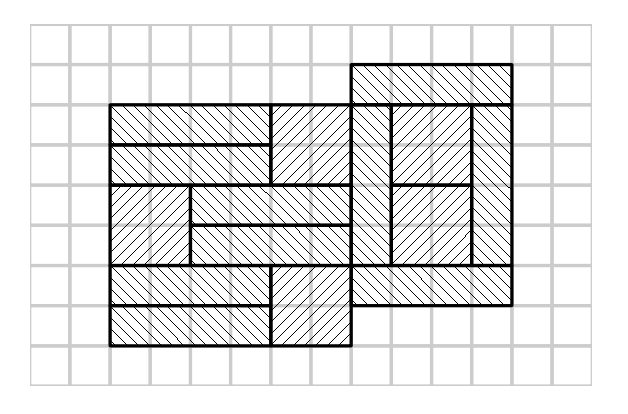
\includegraphics[scale=0.5]{tiles}
	      \end{center}

	      Lösung:
	      \begin{enumerate}
		      \item Das Ersetzen eines \( 1 \times 4 \) Stückes durch ein \( 2 \times 2 \) ist nur möglich, wenn in der
				Ausgangsform \( \geq 2 \) \( 1 \times 4 \) Stücke verwendet wurden und sich mindestens ein \( 2 \times 4 \).
				Rechteck in der Form befindet.
		            \begin{center}
			            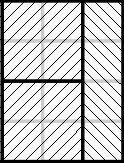
\includegraphics[scale=0.5]{tiles_small}
		            \end{center}
		            Denn falls dies nicht der Fall ist, muss eine der Seitenlängen der Ausgansform ungerade sein und kann somit
		            nicht durch Stücke gerader Kantenlänge ersetzt werden.

		            Falls eine Kantenlänge der Ausgangsform ungerade ist, aber \( > 2 \) \( 1 \times 4 \) Stücke werwendet wurden,
		            ist es immer möglich \( 2 \) dieser mit einer Gesamtfläche von \( 2 \cdot (1 \times 4) = 8 \) durch \( 2 \) \( 2 \times 2  \)
		            Stücke zu ersetzen. Denn das fehlerhafte \( 1 \times 4 \) Stück kann mit einem fehlerfreien zu einem
		            gemeinsamen \( 2 \times 4 \) Stück zusammen gelegt werden,
		            welches sich dann durch \( 2 \cdot (2 \times 2) \) Stücke ersetzen lässt.
	      \end{enumerate}
\end{enumerate}
\end{document}